\documentclass[border=10pt]{standalone}
\usepackage{tikz}
\usetikzlibrary{arrows.meta, shapes.geometric, calc}

\begin{document}
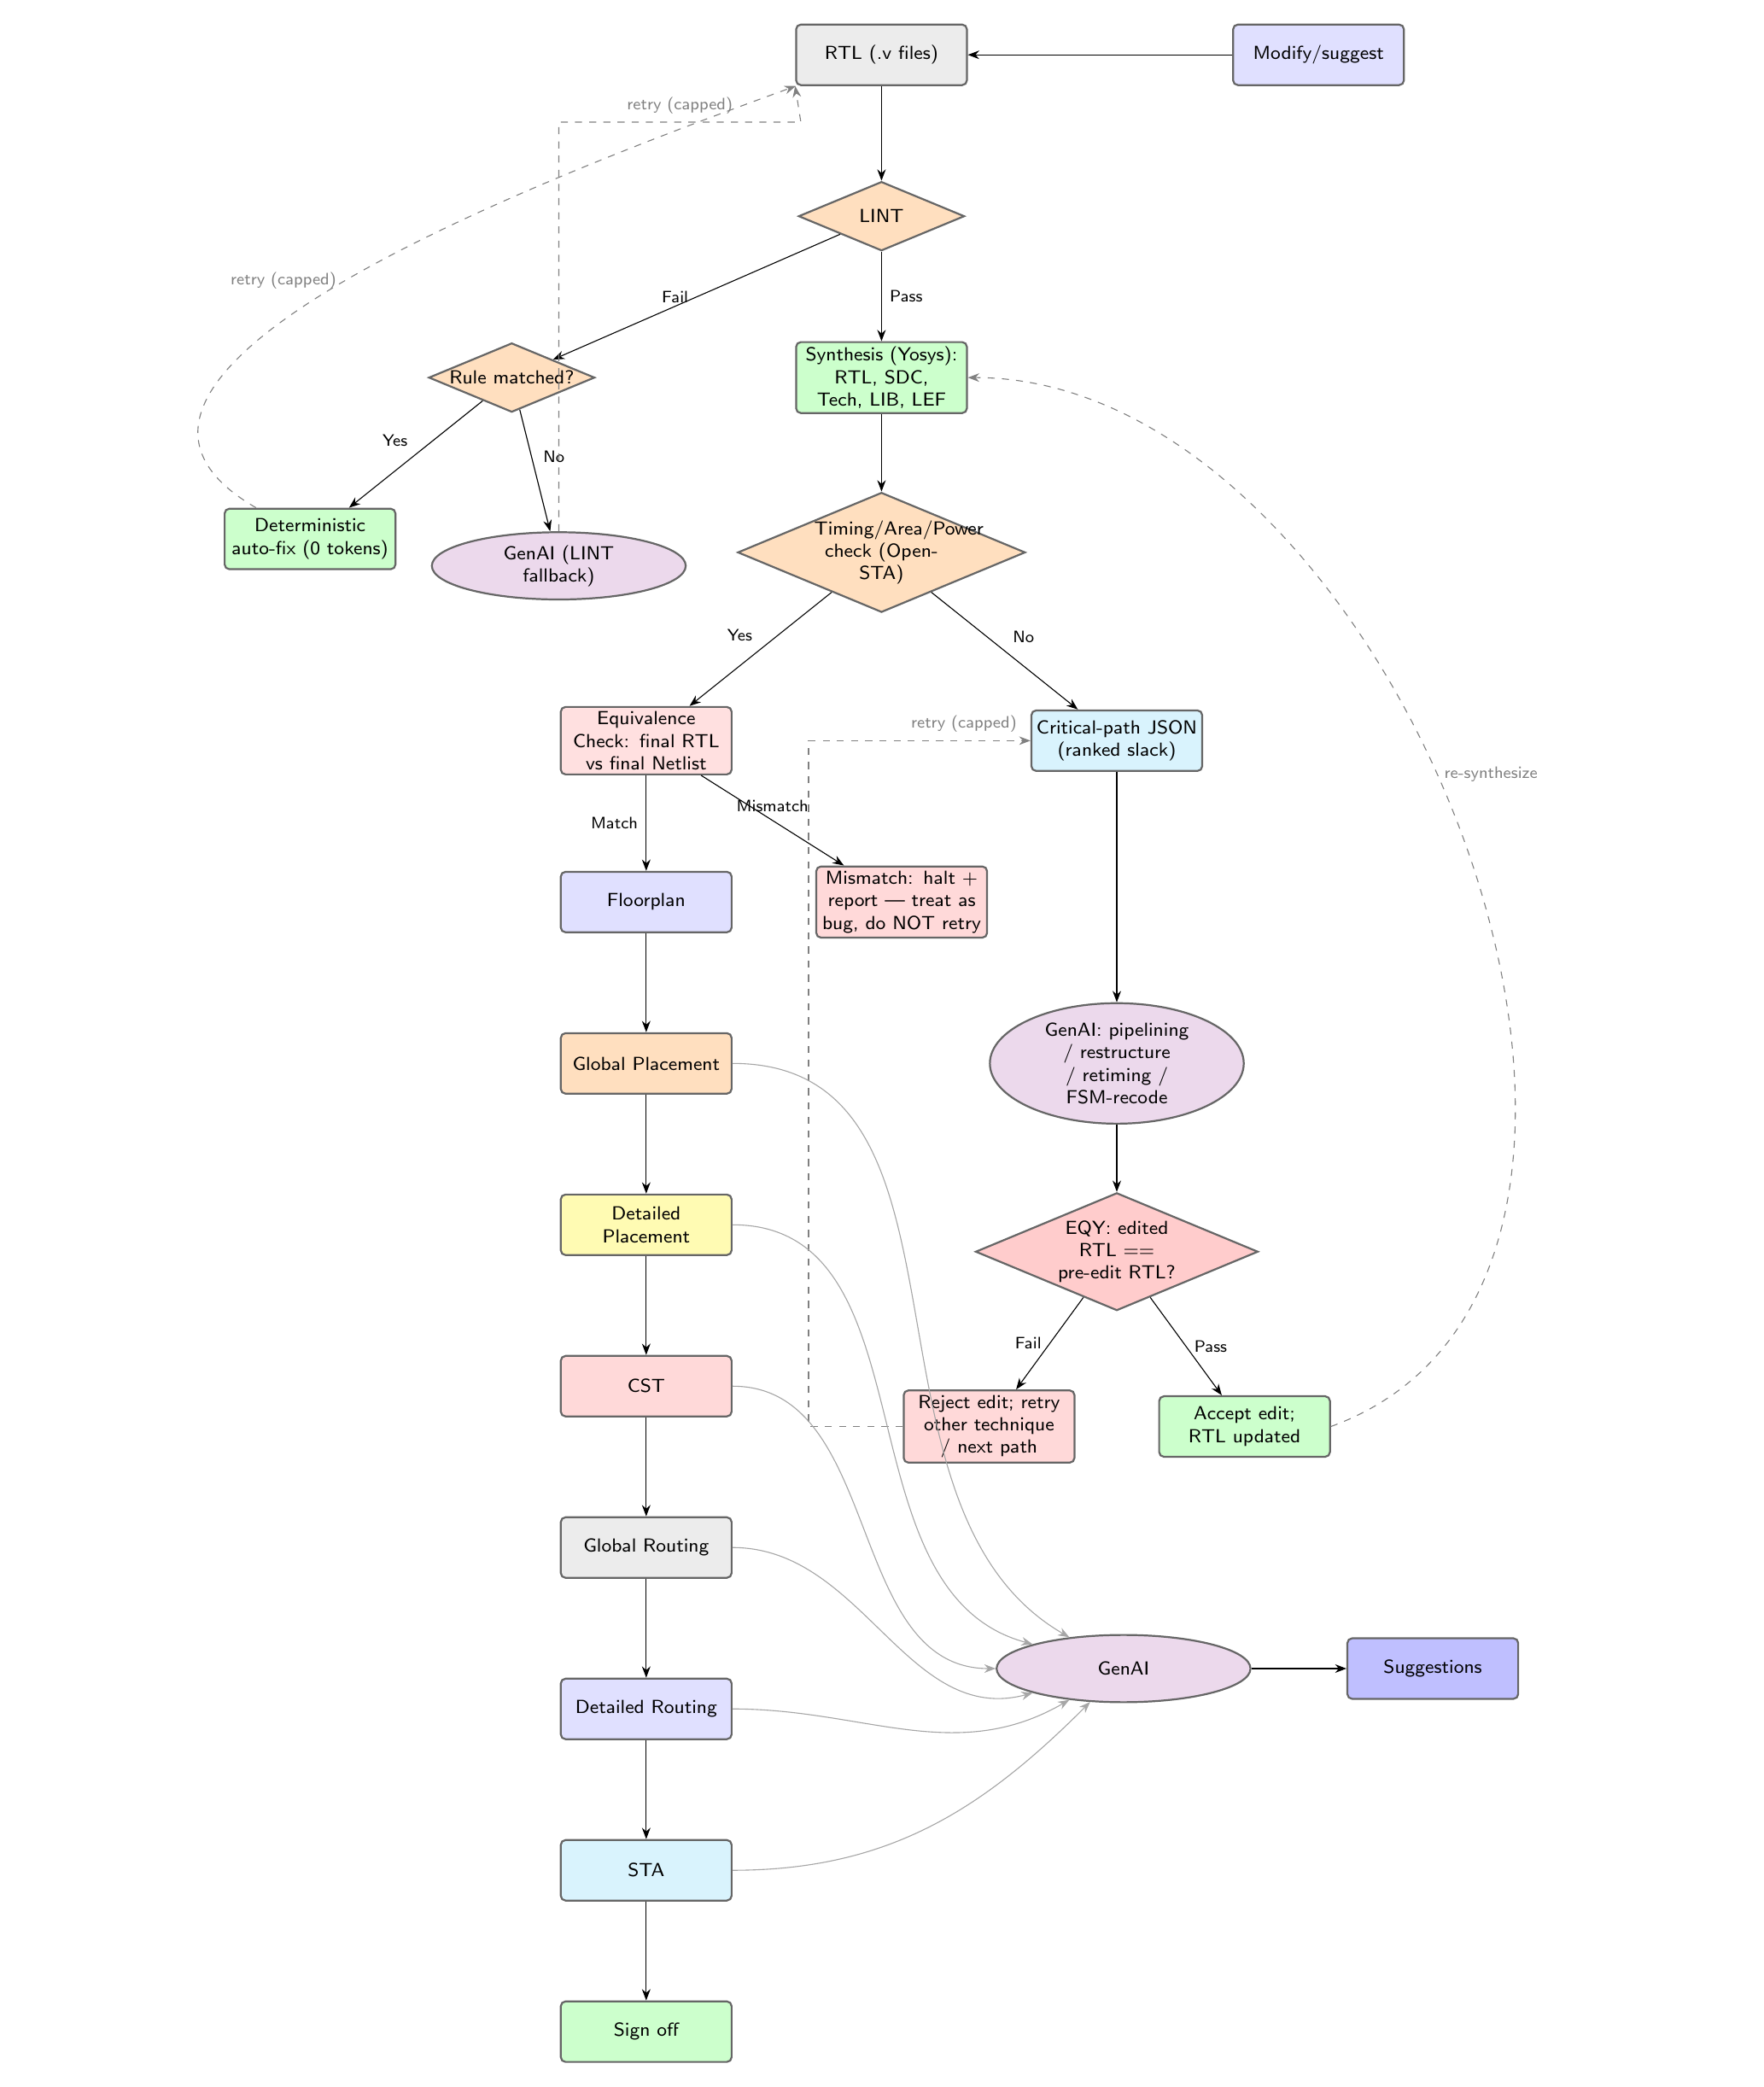
\begin{tikzpicture}[
  font=\sffamily\footnotesize,
  >=Stealth,
  box/.style={rectangle, rounded corners=2pt, draw=black!60, thick, fill=#1,
              minimum height=9mm, text width=24mm, align=center, inner sep=2pt},
  dia/.style={diamond, draw=black!60, thick, fill=#1, aspect=2.4,
              minimum height=9mm, text width=20mm, align=center, inner sep=0pt},
  ell/.style={ellipse, draw=black!60, thick, fill=#1,
              minimum height=10mm, text width=26mm, align=center, inner sep=1pt},
  lbl/.style={font=\sffamily\scriptsize},
  ->,
]

% ================= NODES (explicit coords, cm) =================
\node[box=gray!15]              (rtl)      at (0,0)        {RTL (.v files)};
\node[box=blue!12]              (modsug)   at (6.5,0)      {Modify/suggest};

\node[dia=orange!25]            (lint)     at (0,-2.4)     {LINT};

\node[dia=orange!25]            (rulematch)at (-5.5,-4.8)  {Rule matched?};
\node[box=green!20]             (autofix)  at (-8.5,-7.2)  {Deterministic auto-fix (0 tokens)};
\node[ell=violet!15]            (genailint)at (-4.8,-7.6)  {GenAI (LINT fallback)};

\node[box=green!20]             (synth)    at (0,-4.8)     {Synthesis (Yosys): RTL, SDC, Tech, LIB, LEF};
\node[dia=orange!25]            (tap)      at (0,-7.4)     {Timing/Area/Power check (OpenSTA)};

\node[box=red!12]               (eqfinal)  at (-3.5,-10.2) {Equivalence Check: final RTL vs final Netlist};
\node[box=blue!12]              (floorplan)at (-3.5,-12.6) {Floorplan};

\node[box=cyan!15]              (cpjson)   at (3.5,-10.2)  {Critical-path JSON (ranked slack)};
\node[box=red!15]               (mismatch) at (0.3,-12.6)  {Mismatch: halt + report --- treat as bug, do NOT retry};
\node[ell=violet!15]            (genaiedit)at (3.5,-15.0)  {GenAI: pipelining / restructure / retiming / FSM-recode};
\node[dia=red!20]               (eqedit)   at (3.5,-17.8)  {EQY: edited RTL == pre-edit RTL?};
\node[box=red!15]               (reject)   at (1.6,-20.4)  {Reject edit; retry other technique / next path};
\node[box=green!20]             (accept)   at (5.4,-20.4)  {Accept edit; RTL updated};

% PnR chain (left column, continuing down from Floorplan)
\node[box=orange!25]            (gp)       at (-3.5,-15.0) {Global Placement};
\node[box=yellow!30]            (dp)       at (-3.5,-17.4) {Detailed Placement};
\node[box=red!15]               (cts)      at (-3.5,-19.8) {CST};
\node[box=gray!15]              (gr)       at (-3.5,-22.2) {Global Routing};
\node[box=blue!12]              (dr)       at (-3.5,-24.6) {Detailed Routing};
\node[box=cyan!15]              (sta)      at (-3.5,-27.0) {STA};
\node[box=green!20]             (signoff)  at (-3.5,-29.4) {Sign off};

\node[ell=violet!15]            (genai2)   at (3.6,-24.0)  {GenAI};
\node[box=blue!25]              (suggest)  at (8.2,-24.0)  {Suggestions};

% ================= EDGES =================
\draw (rtl) -- (lint);
\draw (modsug) -- (rtl);

\draw (lint) -- node[lbl, left]{Fail} (rulematch);
\draw (lint) -- node[lbl, right]{Pass} (synth);

\draw (rulematch) -- node[lbl, above left]{Yes} (autofix);
\draw (rulematch) -- node[lbl, above right]{No} (genailint);

\draw[dashed, gray] (autofix) to[out=150,in=200] node[lbl,gray,left,pos=0.5]{retry (capped)} (rtl);
\draw[dashed, gray] (genailint.north) -- (-4.8,-1.0) -- node[lbl,gray,above,pos=0.5]{retry (capped)} (-1.2,-1.0) -- (rtl.south west);

\draw (synth) -- (tap);

\draw (tap) -- node[lbl, above left]{Yes} (eqfinal);
\draw (tap) -- node[lbl, above right]{No} (cpjson);

\draw (eqfinal) -- node[lbl, left]{Match} (floorplan);
\draw (eqfinal) -- node[lbl, above]{Mismatch} (mismatch);

\draw (cpjson) -- (genaiedit);
\draw (genaiedit) -- (eqedit);
\draw (eqedit) -- node[lbl, left]{Fail} (reject);
\draw (eqedit) -- node[lbl, right]{Pass} (accept);

\draw[dashed, gray] (reject.west) -- ++(-1.4,0) |- node[lbl,gray,pos=0.85,above]{retry (capped)} (cpjson.west);
\draw[dashed, gray] (accept.east) to[out=20,in=0] node[lbl,gray,right,pos=0.55]{re-synthesize} (synth.east);

\draw (floorplan) -- (gp);
\draw (gp) -- (dp);
\draw (dp) -- (cts);
\draw (cts) -- (gr);
\draw (gr) -- (dr);
\draw (dr) -- (sta);
\draw (sta) -- (signoff);

\draw[-{Stealth}, gray!70] (gp.east) to[out=0,in=150] (genai2);
\draw[-{Stealth}, gray!70] (dp.east) to[out=0,in=165] (genai2);
\draw[-{Stealth}, gray!70] (cts.east) to[out=0,in=180] (genai2);
\draw[-{Stealth}, gray!70] (gr.east) to[out=0,in=195] (genai2);
\draw[-{Stealth}, gray!70] (dr.east) to[out=0,in=210] (genai2);
\draw[-{Stealth}, gray!70] (sta.east) to[out=0,in=225] (genai2);
\draw (genai2) -- (suggest);

\end{tikzpicture}
\end{document}
